%! suppress = MissingImport
%! suppress = MissingLabel
%! suppress = LineBreak

% CLI args https://tex.stackexchange.com/a/1501
\newif\ifhandout
\input{flags}

%! suppress = MissingLabel
%! suppress = DocumentclassNotInRoot
%! suppress = DiscouragedUseOfDef

% * Make friends tikz & colors
%   https://en.wikibooks.org/wiki/LaTeX/Colors
% * To enable vertical top alignment globally
%   https://tex.stackexchange.com/questions/9889/positioning-content-at-the-top-of-a-beamer-slide-by-default
% * Set handout from CLI
%   https://tex.stackexchange.com/a/1501
\ifhandout
\documentclass[usenames, dvipsnames, handout]{beamer} % https://tex.stackexchange.com/questions/224091/beamer-how-to-disable-pause-temporarily
\else
\documentclass[usenames, dvipsnames]{beamer}
\fi
% ------------------------------------------------

% Graphics
\usepackage{color}
\usepackage{tabularx}
\usepackage{tikz}
% https://tikz.dev/tikz-graphs
\usetikzlibrary{positioning, shapes.geometric, arrows, automata, graphs}
\tikzset{
    expr/.style={ellipse, draw=gray!60, fill=gray!5, very thick, minimum size=7mm, yshift=0.7cm},
    hexpr/.style={ellipse, draw=gray!60, fill=blue!15, very thick, minimum size=7mm, yshift=0.7cm},
    stmt/.style={rectangle, draw=gray!60, fill=gray!5, very thick, minimum size=5mm, yshift=0.7cm},
    decl/.style={rectangle, draw=blue!60, fill=gray!5, very thick, minimum size=5mm, yshift=0.7cm},
    hdecl/.style={rectangle, draw=blue!60, fill=blue!15, very thick, minimum size=5mm, yshift=0.7cm},
    subtree/.style={shape border rotate=90, isosceles triangle, draw=gray!60, fill=gray!5, very thick, minimum size=5mm, yshift=0.0cm},
}
\usepackage{blkarray}
\usepackage{graphicx}
\usepackage{forest} % https://tex.stackexchange.com/questions/198405/how-to-change-the-color-of-subtrees-in-tikz-qtree
% ------------------------------------------------

% Math
\usepackage{amsmath, amsfonts}
\usepackage{amssymb}
\usepackage{proof}
\usepackage{mathrsfs}
% Crossed-out symbols
% https://tex.stackexchange.com/questions/75525/how-to-write-crossed-out-math-in-latex
\usepackage[makeroom]{cancel}
\usepackage{mathtools}
% ------------------------------------------------

% Additional font sizes
% https://www.overleaf.com/learn/latex/Questions/How_do_I_adjust_the_font_size%3F
\usepackage{moresize}
% Additional colors
% https://www.overleaf.com/learn/latex/Using_colours_in_LaTeX
\usepackage{xcolor}
% Textual math symbols
\usepackage{textcomp}
% ------------------------------------------------

% Language
\usepackage[utf8] {inputenc}
\usepackage[T2A] {fontenc}
\usepackage[english, russian] {babel}
\usepackage{indentfirst, verbatim}
\usetikzlibrary{cd, babel}
% ------------------------------------------------

% Fonts: https://sites.math.washington.edu/~reu/docs/latex_symbols.pdf
\usepackage{stmaryrd}
\usepackage{cmbright}
\usepackage{wasysym}
\usepackage[weather]{ifsym} % https://tex.stackexchange.com/questions/100424/how-to-use-the-ifsym-package
% https://tex.stackexchange.com/questions/615300/pdflatex-builtin-glyph-names-is-empty
\pdfmapline{=dictsym DictSym <dictsym.pfb}
\pdfmapline{=pigpen <pigpen.pfa}
\usepackage{dictsym}
% ------------------------------------------------

% Code
% * Needs -shell-escape build flag
%   https://tex.stackexchange.com/questions/99475/how-to-invoke-latex-with-the-shell-escape-flag-in-texstudio-former-texmakerx
% * Set build directory
%   https://tex.stackexchange.com/questions/339931/latex-minted-package-using-custom-output-directory-build
\usepackage{minted}
\setminted{xleftmargin=\parindent, autogobble, escapeinside=\#\#}
% ------------------------------------------------

% Template
\usetheme{CambridgeUS}
\usecolortheme{dolphin}
% https://tex.stackexchange.com/questions/231439/beamer-how-to-make-font-larger-for-page-numbers
\setbeamerfont{headline}{size=\scriptsize}
\setbeamerfont{footline}{size=\scriptsize}
% Remove heddline
% https://tex.stackexchange.com/questions/33146/how-could-i-remove-a-header-in-a-beamer-presentation
%\setbeamertemplate{headline}{}
% Slide sizes
% https://tex.stackexchange.com/questions/56768/how-to-set-a-small-default-font-size-with-beamer
%\geometry{paperwidth=140mm,paperheight=105mm} % 4:3
\geometry{paperwidth=168mm,paperheight=105mm} % 16:10
% Remove navigation bar
% https://stackoverflow.com/questions/3210205/how-to-get-rid-of-navigation-bars-in-beamer
\beamertemplatenavigationsymbolsempty
% ------------------------------------------------

% Bullets
% https://9to5science.com/change-bullet-style-formatting-in-beamer
% https://tex.stackexchange.com/questions/185742/i-need-to-change-color-of-beamer-itemize-and-subitem-separately
\setbeamertemplate{itemize item}{\scriptsize\raise1.25pt\hbox{\donotcoloroutermaths$\blacktriangleright$}}
\setbeamertemplate{itemize subitem}{\scriptsize\raise1.5pt\hbox{\donotcoloroutermaths$\blacktriangleright$}}
\setbeamertemplate{itemize subsubitem}{\tiny\raise1.5pt\hbox{\donotcoloroutermaths$\blacktriangleright$}}
\setbeamertemplate{enumerate item}{\insertenumlabel.}
\setbeamertemplate{enumerate subitem}{\insertenumlabel.\insertsubenumlabel}
\setbeamertemplate{enumerate subsubitem}{\insertenumlabel.\insertsubenumlabel.\insertsubsubenumlabel}
% ------------------------------------------------

% Table of contents format
% https://tex.stackexchange.com/questions/642927/format-table-of-contents-in-beamer
\setbeamertemplate{section in toc}{%
        {\color{blue}\inserttocsectionnumber.}
    \inserttocsection\par%
}
\setbeamertemplate{subsection in toc}{%
        {\color{blue}\hspace{1em}\scriptsize\raise1.25pt\hbox{\donotcoloroutermaths$\blacktriangleright$}}
    \inserttocsubsection\par%
}
\setbeamertemplate{subsubsection in toc}{%
        {\color{blue}\hspace{2em}\tiny\raise1.25pt\hbox{\donotcoloroutermaths$\blacktriangleright$}}
    \inserttocsubsubsection\par%
}
% ------------------------------------------------

% Misc
\usepackage{multicol}
\usepackage{hyperref}
\usepackage{soul} % https://tex.stackexchange.com/questions/23711/strikethrough-text
% ------------------------------------------------

% Fix \pause for amsmath package envs (black black magic)
% https://tex.stackexchange.com/questions/16186/equation-numbering-problems-in-amsmath-environments-with-pause/75550#75550
% https://tex.stackexchange.com/questions/6348/problem-with-beamers-pause-in-alignments
%! suppress = Makeatletter
\makeatletter
\let\save@measuring@true\measuring@true
\def\measuring@true{%
    \save@measuring@true
    \def\beamer@sortzero##1{\beamer@ifnextcharospec{\beamer@sortzeroread{##1}}{}}%
    \def\beamer@sortzeroread##1<##2>{}%
    \def\beamer@finalnospec{}%
}
%! suppress = Makeatletter
\makeatother
% ------------------------------------------------

% Sections
\newcommand{\sectionplan}[1]{\section{#1}%
    \begin{frame}[noframenumbering]{Содержание}
        \tableofcontents[currentsection]
    \end{frame}
}
\newcommand{\subsectionplan}[1]{\subsection{#1}%
    \begin{frame}[noframenumbering]{Содержание}
        \tableofcontents[currentsubsection]
    \end{frame}
}
% ------------------------------------------------

% Footnotes
\renewcommand{\thefootnote}{\arabic{footnote}}
\renewcommand{\thempfootnote}{\arabic{mpfootnote}}
% https://tex.stackexchange.com/questions/28465/multiple-footnotes-at-one-point
\usepackage{fnpct}
% ------------------------------------------------

% Links
% Colors also links on slide foot.
%\hypersetup{
%    colorlinks=true,
%    citecolor=blue,
%    linkcolor=blue,
%    urlcolor=blue
%}
% ------------------------------------------------

% Appendix
% Slide numbers
% https://tex.stackexchange.com/questions/70448/dont-count-backup-slides
\usepackage{appendixnumberbeamer}
\newcommand{\backupbegin}{
    \newcounter{framenumbervorappendix}
    \setcounter{framenumbervorappendix}{\value{framenumber}}
}
\newcommand{\backupend}{
    \addtocounter{framenumbervorappendix}{-\value{framenumber}}
    \addtocounter{framenumber}{\value{framenumbervorappendix}}
}
% ------------------------------------------------

% Custom commands
% * Decor
\newcommand{\newtopic}[0]{$+$} % item: new topic on "in previous series"
\newcommand{\then}{$\Rightarrow$} % item: consequences
\newcommand{\pop}[0]{\SunCloud} %item:  general eduation
\newcommand{\popslide}[0]{(\pop)}
\newcommand{\advanced}[0]{$\varhexstar$} % item: advanced science
\newcommand{\advancedslide}[0]{(\advanced)}
\newcommand{\practical}[0]{\dstechnical} % item: practical programming notions
\newcommand{\practicalslide}[0]{(\practical)}
\newcommand{\todo}[0]{todo} % item: question
\newcommand{\answer}[0]{\Lightning} % item: answer to the previous question
\newcommand{\eg}[0]{e.g.} % item: example
\newcommand{\defi}[0]{$\Delta$} % item: definition on smth
\newcommand{\textdefi}[1]{\textbf{#1}}
\newcommand{\positive}{$+$} % item: pros
\newcommand{\negative}{{\color{red} $-$}} % item: cons
\newcommand%! suppress = EscapeHashOutsideCommand
\NB[1][0.3]{N\kern-#1em{B}} % default kern amount: -0.3em
\renewcommand{\emph}[1]{{\color{blue} \textit{#1}}}
\newcommand{\vocab}[1]{\textbf{#1}} % item: important new word
% * Lambda calculi
\newcommand{\comb}[1]{\mathbf{#1}} % defined combinator
\newcommand{\term}[1]{\mathbf{#1}} % predefined lambda-term reference
\newcommand{\termdef}{\coloneqq} % lamda term binding
\newcommand{\step}{\rightsquigarrow} % reduction step
\newcommand{\sstep}{\twoheadrightarrow} % multiple steps reduction
\newcommand{\ap}{~} % lambda-term application
\newcommand{\subst}[3]{\left[#2 \mapsto #3 \right] #1} % substitution
\newcommand{\eqbeta}{=_\beta} % beta equality
\newcommand{\eqeta}{=_\eta} % eta-equality
\newcommand{\eqt}{=} % tree-equality of terms
\newcommand{\tlist}[1]{\term{[}#1\term{]}} % list-term
% * Legacy
%\newcommand{\err}[0]{\textcolor{red}{ошибка}} % compilation error

% ------------------------------------------------

% Speaker notes
% https://tex.stackexchange.com/questions/114219/add-notes-to-latex-beamer
% https://tex.stackexchange.com/questions/35444/split-beamer-notes-across-multiple-notes-pages/35496#35496
%\setbeameroption{show notes on second screen=right} % enable speaker notes
%--------------------------------------

\author[]{Андрей Стоян, Илья Колегов, Дмитрий Халанский}
\institute[MSE ITMO]{MSE ITMO}

\setminted{xleftmargin=\parindent, autogobble, escapeinside=??}

\title[2. Параметрический полиморфизм]{2. Параметрический полиморфизм}
\author{Андрей Стоян}
\institute[ИПКН ИТМО]{ИПКН ИТМО}

\date{осень 2025}

\begin{document}

    \mymaketitle

    \begin{frame}[noframenumbering]{Содержание}
        \tableofcontents
    \end{frame}

    \sectionplan{Параметрический полиморфизм в языке}

    \begin{frame}[fragile]{Пары Чёрча}
        \pause
        \begin{align*}
            &Pair : * \rightarrow * \rightarrow * \\
            &Pair = \lambda \tau^*~\sigma^*\ldotp\forall \gamma\ldotp(\tau\rightarrow\sigma\rightarrow\gamma)\to\gamma \\
            &pair : \forall \alpha~\beta\ldotp\alpha \rightarrow \beta \rightarrow Pair~\alpha~\beta \\
            &pair = \Lambda \alpha^*~\beta^*\ldotp\lambda x^\alpha~y^\beta\ldotp(\Lambda \gamma^*\ldotp\lambda f^{\alpha\rightarrow\beta\rightarrow\gamma}\ldotp f~x~y) \\
            &fst : \forall \alpha~\beta\ldotp Pair~\alpha~\beta\rightarrow \alpha \\
            &fst = \Lambda \alpha^*~\beta^*\ldotp\lambda p^{Pair~\alpha~\beta}\ldotp p~\alpha~(\mathbf{K}\ap\alpha\ap\beta)
        \end{align*}
    \end{frame}

    \begin{frame}[fragile]{\mintinline{haskell}{Proxy}}
        \pause
        \begin{minted}[escapeinside=??]{haskell}
            data Proxy a = Proxy

            id :: Proxy a -> a -> a
            ghci> :t id (Proxy :: Proxy Int)
            id (Proxy :: Proxy Int) :: Int -> Int

            id (Proxy :: Proxy ?\framebox{a}?) x = (x :: ?\framebox{a}?)
        \end{minted}

        \pause\hspace{2em}
        \begin{minted}{haskell}
            id :: proxy a -> a -> a
            id (_ :: proxy a) x = (x :: a)

            ghci> :t id (undefined :: Proxy Int)
            id (undefined :: Proxy Int) :: Int -> Int
        \end{minted}
    \end{frame}

    \begin{frame}[fragile]{First-class polymorphism}
        \pause
        \begin{minted}{haskell}
            f :: (forall a . a -> a) -> (Int, Char)
            f g = (g @Int 42, g @Char 'a') -- универсальная аппликация для наглядности
            ghci> f (\x -> x)
        \end{minted}

        \pause\hspace{2em}
        \begin{minted}{haskell}
            suc :: (forall a . (a -> a) -> a -> a) -> (a -> a) -> a -> a
            suc n s z = s (n s z)
        \end{minted}
        \pause\hspace{2em}
        Какой ранг имеет тип \mintinline{haskell}|Int -> (forall a . a -> a)|?
    \end{frame}

    \begin{frame}[fragile]{Числа Чёрча}
        \pause
        \begin{minted}{haskell}
            newtype Church = Church (forall a . (a -> a) -> a -> a)
            (+) :: Church -> Church -> Church -- rank 1
        \end{minted}

        \pause\hspace{2em}
        \begin{minted}{kotlin}
            interface Church {
                fun <a> fold(s: (a) -> a, z: a): a
            }
            fun plus(n: Church, m: Church): Church =
                object : Church {
                override fun <a> fold(s: (a) -> a, z: a): a =
                    n.fold(s, m.fold(s, z))
                }
        \end{minted}
    \end{frame}

    \begin{frame}[fragile]{Impredicative apprication}
        \pause
        \begin{minted}{haskell}
            runST :: (forall s. ST s a) -> a
            ($) :: forall a b . (a -> b) -> a -> b
            foo = runST $ ... -- типизируется только с ImpredicativeTypes
        \end{minted}
    \end{frame}

    \begin{frame}[fragile]{ST-trick}
        \pause
        \begin{minted}{haskell}
            newtype ST s a = ST (IO a)
            runST :: (forall s. ST s a) -> a

            sumTo :: Int -> Int
            sumTo n = runST do
              ref <- newSTRef 0
              forM [0..n] \i -> modifySTRef ref (+ i)
              readSTRef ref
        \end{minted}

        \pause\hspace{2em}
        \begin{minted}{haskell}
            newSTRef :: a -> ST s (Ref s a)
            ghci> runST (newSTRef 0) :: Ref s Int -- ошибка
        \end{minted}
    \end{frame}

    \begin{frame}[fragile]{Higher-order/kinded polymorphism}
        \pause
        \begin{minted}{haskell}
            newtype Fix f = Fix (f (Fix f))
            cata :: forall (f :: Type -> Type) a . Functor f => (f a -> a) -> Fix f -> a
        \end{minted}
    \end{frame}

    \begin{frame}[fragile]{Обобщённые алгебраические типы данных (GADTs)}
        \pause
        \begin{minted}{haskell}
            data Expr = Const Int | IsZero Expr | If Expr Expr Expr
        \end{minted}

        \pause\hspace{2em}
        \begin{minted}{haskell}
            data Expr where
              Const :: Int -> Expr
              IsZero :: Expr -> Expr
              If :: Expr -> Expr -> Expr -> Expr
        \end{minted}

        \pause\hspace{2em}
        \begin{minted}{haskell}
            data List (elem :: Type) where
              Nil :: List a
              Cons :: a -> List a -> List a
        \end{minted}
    \end{frame}

    \begin{frame}[fragile]{Обобщённые алгебраические типы данных (GADTs)}
        \pause
        \begin{minted}{haskell}
            data Expr ty where
              Const :: Int -> Expr Int
              IsZero :: Expr Int -> Expr Bool
              If :: forall ty . Expr Bool -> Expr ty -> Expr ty -> Expr ty
        \end{minted}

        \pause\hspace{2em}
        \begin{minted}[escapeinside=??]{haskell}
            eval :: Expr ty -> ty
            eval = \case
              Const x  -> x         -- ty ?$\sim$? Int
              IsZero t -> eval t == 0 -- ty ?$\sim$? Bool
              If c t e -> if eval c then eval t else eval e
        \end{minted}
    \end{frame}

    \begin{frame}[fragile]{Структуры на уровне типов, data promotion}
        \pause
        \begin{minted}{haskell}
            data Zero
            data Suc n
        \end{minted}

        \pause\hspace{2em}
        \begin{minted}{haskell}
            data Vec (size :: Type) (elem :: Type) where
              VNil :: Vec Zero a
              VCons :: a -> Vec n a -> Vec (Suc n) a

            example :: Vec (Suc (Suc Zero)) Int
            example = VCons 1 (VCons 2 VNil)
        \end{minted}

        \pause\hspace{2em}
        \begin{minted}{haskell}
            vzip :: Vec n a -> Vec n b -> Vec n (a, b)
            vzip VNil VNil = VNil                                      -- n ?$\sim$? Zero
            vzip (VCons x xs) (VCons y ys) = VCons (x, y) (vzip xs ys) -- n ?$\sim$? Suc n'
        \end{minted}
    \end{frame}

    \begin{frame}[fragile]{Структуры на уровне типов, data promotion}
        \pause
        \begin{minted}{haskell}
            type data Nat = Zero | Suc Nat
        \end{minted}

        \pause\hspace{2em}
        \begin{minted}{haskell}
            data Vec (size :: Nat) (elem :: Type) where
              VNil :: Vec Zero a
              VCons :: a -> Vec n a -> Vec (Suc n) a
        \end{minted}

        \pause\hspace{2em}
        \begin{minted}{haskell}
            data Nat = Zero | Suc Nat
            ghci> :k Suc :: Nat -> Nat -- тут понятно что Suc используется как тип
        \end{minted}
    \end{frame}

    \begin{frame}[fragile]{Data promotion}
        \begin{tabular}{|c|c|c|}
            \hline
            Term                                   & Type                                            & Kind                                            \\
            \hline
            \mintinline{haskell}|Zero|             & \mintinline{haskell}|Nat|                       & \mintinline{haskell}|Type|                      \\
            \mintinline{haskell}|[Zero, Suc Zero]| & \mintinline{haskell}|[Nat]|                     & \mintinline{haskell}|Type|                      \\
            \mintinline{haskell}|[]|               & \mintinline{haskell}|forall a. [a]|             & \mintinline{haskell}|Type|                      \\
            \mintinline{haskell}|(:)|              & \mintinline{haskell}|forall a. a -> [a] -> [a]| & \mintinline{haskell}|Type|                      \\
            & \mintinline{haskell}|'Suc 'Zero|                & \mintinline{haskell}|Nat|                       \\
            & \mintinline{haskell}|'['Zero, 'Suc 'Zero]|      & \mintinline{haskell}|[Nat]|                     \\
            & \mintinline{haskell}|'[Int, Double]|            & \mintinline{haskell}|[Type]|                    \\
            & \mintinline{haskell}|'[]|                       & \mintinline{haskell}|forall k. [k]|             \\
            & \mintinline{haskell}|'(:)|                      & \mintinline{haskell}|forall k. k -> [k] -> [k]| \\
            \hline
        \end{tabular}
    \end{frame}

    \begin{frame}[fragile]{HList}
        \pause
        \begin{minted}{haskell}
            data HList (tys :: [Type]) where
              HNil :: HList '[]
              HCons :: ty -> HList tys -> HList (ty ': tys)

            example :: HList '[Int, Bool, Double]
            example = HCons 42 $ HCons True $ HCons 12.5 HNil
        \end{minted}
    \end{frame}

    \begin{frame}[fragile]{PolyKinds}
        \pause
        \begin{minted}{haskell}
            newtype Tagged (tag :: k) (a :: Type) = Tagged a
            ghci> :t Tagged
            Tagged :: forall k (tag :: k) a. a -> Tagged tag a

            example :: Tagged ("dbId" :: Symbol) Int
            example = Tagged 42
        \end{minted}
    \end{frame}

    \begin{frame}[fragile]{Типы и канды --- одно}
        \pause
        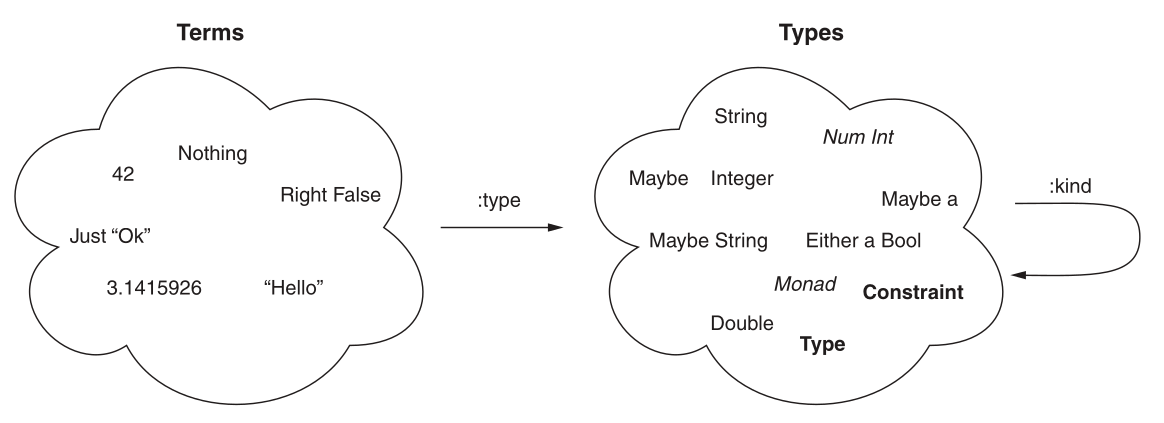
\includegraphics[width=0.99\textwidth]{figs/types-eq-kinds}
    \end{frame}

    \sectionplan{Реализация параметрического полиморфизма}

    \begin{frame}[fragile]{Использование виртуальной таблицы свойств типов}
        \begin{figure}
            \centering
            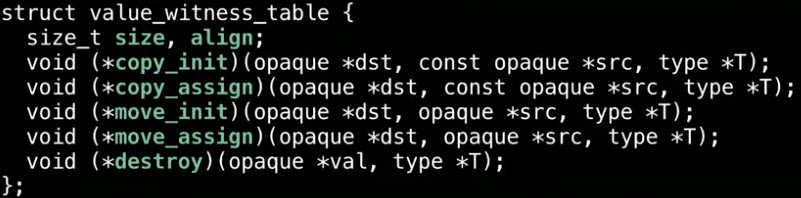
\includegraphics[width=0.7\textwidth]{figs/swift-witness-table}
        \end{figure}
        \begin{figure}
            \centering
            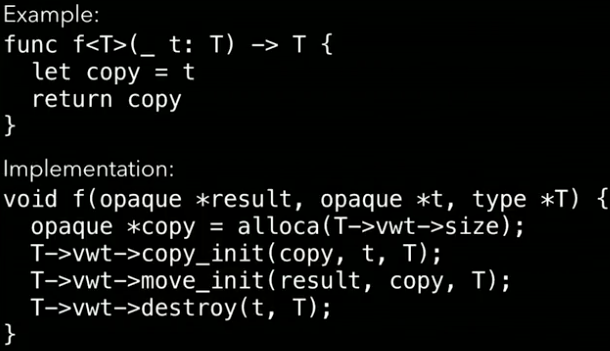
\includegraphics[width=0.5\textwidth]{figs/swift-generated-code}
        \end{figure}
    \end{frame}

    \sectionplan{Полиморфизм по конвенции вызова}

    \begin{frame}[fragile]{Виды значений в Haskell с примерами}
        \pause
        \begin{center}
            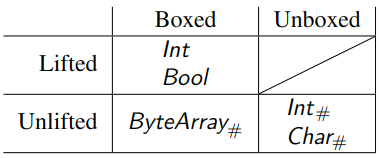
\includegraphics[width=0.5\textwidth]{figs/haskell-value-kinds}
        \end{center}
    \end{frame}

    \begin{frame}[fragile]{Unboxed tuples}
         \pause
         \begin{minted}{haskell}
            divMod# :: Int -> Int -> (# Int, Int #)
            case divMod# n k of (# quot, rem #) -> ...
         \end{minted}

        \pause\hspace{2em}
         \begin{minted}{haskell}
            (# A, (# B, C #)) ?$\equiv$? (# #( A, B #), C #) ?$\equiv$? (# A, B, C #)
         \end{minted}
    \end{frame}

    \begin{frame}[fragile]{Классификация значений по runtime представлению}
        \pause
        \begin{minted}{haskell}
            TYPE :: RuntimeRep -> Type

            data Levity = Lifted | Unlifted

            data RuntimeRep = BoxedRep Levity
                            | IntRep | DoubleRep
                            | TupleRep [RuntimeRep]
                            | SumRep [RuntimeRep]
                            | ...

            type LiftedRep = BoxedRep Lifted

            type Type = TYPE LiftedRep
        \end{minted}
    \end{frame}

    \begin{frame}[fragile]{Примеры}
        \pause
        \begin{itemize}
            \item \mintinline{haskell}|Int ::?\pause? TYPE (BoxedRep Lifted)| или \mintinline{haskell}|:: Type|
            \item \mintinline{haskell}|IntRep| и \mintinline{haskell}|DoubleRep| соответствуют представлению численных констант (в зависимости от архитектуры процессора, целые числа и числа с плавающей запятой может быть необходимо располагать в различных специальных регистрах)\\ \mintinline{haskell}|Int# ::?\pause? TYPE IntRep|
            \item \mintinline{haskell}|Maybe Int ::?\pause? Type|
            \item \mintinline{haskell}|Maybe ::?\pause? Type -> Type|
            \item \mintinline{haskell}|TupleRep| и \mintinline{haskell}|SumRep| --- unboxed алгебраические типы, представления параметризованы представлениями хранимых значений\\
            \mintinline{haskell}|(# Int, Bool #) ::?\pause? TYPE (TupleRep '[LiftedRep, LiftedRep])|
            \item Для простоты, типы вложенных кортежей не унифицируются
            \begin{minted}{haskell}
        (# Int#, (# Int, Double# #) #)
          ::?\pause? TYPE (TupleRep '[IntRep, TupleRep '[LiftedRep, DoubleRep]])
            \end{minted}
        \end{itemize}
    \end{frame}

    \begin{frame}[fragile]{Representation polymorphism}
        \pause
        \begin{minted}{haskell}
            ghci> :k (->)
            (->) :: forall {q :: RuntimeRep} {r :: RuntimeRep}. TYPE q -> TYPE r -> Type
        \end{minted}

        \pause\hspace{2em}
        \begin{minted}{haskell}
            ($) :: forall r a (b :: TYPE r). (a -> b) -> a -> b
            f $ ?\framebox{x}? = f x
        \end{minted}

        \pause\hspace{2em}
        \begin{minted}{haskell}
            ($) :: forall ra rb (a :: TYPE ra) (b :: TYPE rb). (a -> b) -> a -> b
            ($) f = f
        \end{minted}
    \end{frame}

\end{document}
